% Created 2018-04-09 lun 18:25
% Intended LaTeX compiler: pdflatex
\documentclass[xcolor={usenames,svgnames,dvipsnames}]{beamer}
\usepackage[utf8]{inputenc}
\usepackage[T1]{fontenc}
\usepackage{graphicx}
\usepackage{grffile}
\usepackage{longtable}
\usepackage{wrapfig}
\usepackage{rotating}
\usepackage[normalem]{ulem}
\usepackage{amsmath}
\usepackage{textcomp}
\usepackage{amssymb}
\usepackage{capt-of}
\usepackage{hyperref}
\usepackage{color}
\usepackage{listings}
\usepackage{mathpazo}
\usepackage{gensymb}
\usepackage{amsmath}
\usepackage{chemarr}%flechas para reacciones químicas (SFER.tex)
\bibliographystyle{plain}
\AtBeginSubsection[]{\begin{frame}[plain]\tableofcontents[currentsubsection,sectionstyle=show/shaded,subsectionstyle=show/shaded/hide]\end{frame}}
\AtBeginSection[]{\begin{frame}[plain]\tableofcontents[currentsection,hideallsubsections]\end{frame}}
\usepackage[emulate=units]{siunitx}
\sisetup{fraction=nice, decimalsymbol=comma, retain-unity-mantissa = false}
\newunit{\wattpeak}{Wp}
\newunit{\watthour}{Wh}
\newunit{\amperehour}{Ah}
\hypersetup{colorlinks=true, linkcolor=Blue, urlcolor=Blue}
\renewcommand{\thefootnote}{\fnsymbol{footnote}}
\beamertemplatenavigationsymbolsempty
\setbeamertemplate{footline}[frame number]
\setbeamercolor{alerted text}{fg=blue!50!black} \setbeamerfont{alerted text}{series=\bfseries}
\usetheme[hideothersubsections]{Goettingen}
\usecolortheme{rose}
\usefonttheme{serif}
\author{Oscar Perpiñán Lamigueiro \\ \url{http://oscarperpinan.github.io}}
\date{}
\title{Geometría Solar}
\subtitle{Energía Solar Fotovoltaica}
\hypersetup{
 pdfauthor={Oscar Perpiñán Lamigueiro \\ \url{http://oscarperpinan.github.io}},
 pdftitle={Geometría Solar},
 pdfkeywords={},
 pdfsubject={},
 pdfcreator={Emacs 25.2.2 (Org mode 9.1.9)}, 
 pdflang={Spanish}}
\begin{document}

\maketitle

\section{Geometría Sol y Tierra}
\label{sec:org0bb1b27}
\subsection{Movimiento Sol-Tierra}
\label{sec:orgbe7a472}

\begin{frame}[label={sec:org415b95b}]{Movimiento terrestre}
\begin{center}
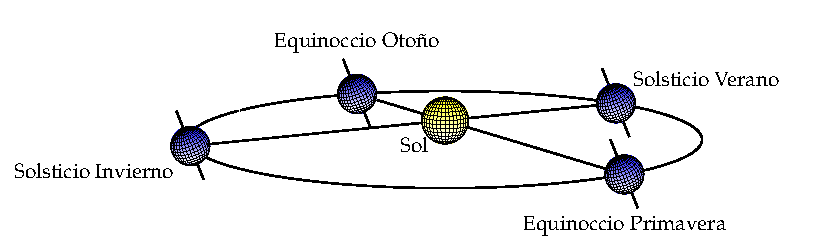
\includegraphics[width=.9\linewidth]{../figs/PlanoEcliptica.pdf}
\end{center}

\begin{itemize}[<+->]
\item La Tierra \alert{gira sobre si misma} alrededor de su eje polar.
\begin{itemize}[<.->]
\item Periodo aproximado: 24 horas.
\end{itemize}

\item La Tierra se mueve \alert{alrededor del Sol} siguiendo una elipse de baja
excentricidad.
\begin{itemize}[<.->]
\item Periodo aproximado: 1 año.

\item Este movimiento está contenido en el llamado \emph{plano de la
eclíptica}
\end{itemize}
\end{itemize}
\end{frame}

\begin{frame}[label={sec:orgf943710}]{Movimiento terrestre}
\begin{center}
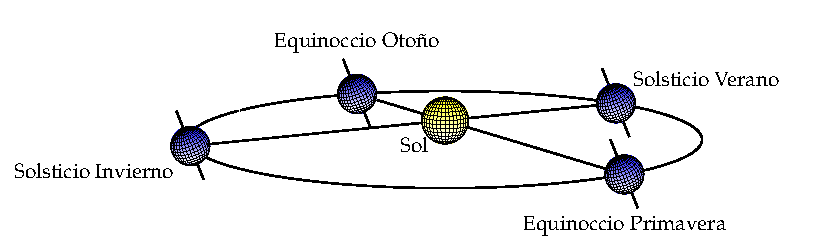
\includegraphics[width=.9\linewidth]{../figs/PlanoEcliptica.pdf}
\end{center}

\begin{itemize}
\item Entre el eje polar y el plano de la eclíptica hay un ángulo constante de \(23,45\degree\).

\item Entre el plano ecuatorial y la linea que une la Tierra y el Sol hay un ángulo variable: \emph{declinación.}
\end{itemize}
\end{frame}

\begin{frame}[label={sec:orgb6ac2d4}]{Distancia Sol-Tierra}
\begin{itemize}
\item Distancia Sol-Tierra
\end{itemize}

\[r=r_{0}\{1+0.017\sin[\frac{2\pi\cdot(d_{n}-93)}{365}]\}\]

\begin{itemize}
\item Distancia promedio
\end{itemize}

\[r_{0}=\SI{1.496e8}{\kilo\metre}=\SI{1}{UA}\]

\begin{itemize}
\item Excentricidad
\end{itemize}

\[\epsilon_{0}=(\frac{r_{0}}{r})^2=1+0,033\cdot\cos(\frac{2\pi
  d_{n}}{365})\]
\end{frame}


\begin{frame}[label={sec:org767f454}]{Estaciones}
\begin{itemize}[<+->]
\item Las estaciones se deben al ángulo entre el plano ecuatorial y el plano de
la eclíptica

\item \alert{Solsticio de junio}
\begin{itemize}[<.->]
\item Declinación máxima.

\item Días más largos en hemisferio Norte (verano)

\item El Sol amanece por el Noreste y anochece por el Noroeste en el
hemisferio Norte.
\end{itemize}

\item \alert{Solsticio de diciembre}
\begin{itemize}[<.->]
\item Declinación mínima.

\item Días más cortos en hemisferio Norte (invierno)

\item El Sol amanece por el Sureste y anochece por el Suroeste en el
hemisferio Norte.
\end{itemize}

\item \alert{Equinoccios}
\begin{itemize}[<.->]
\item Declinación nula

\item La duración de noche y día coincide.

\item El Sol amanece por el Este y anochece por el Oeste.
\end{itemize}
\end{itemize}
\end{frame}

\begin{frame}[label={sec:org2d0edb3}]{Solsticios y equinoccios}
\begin{itemize}
\item \alert{Equinoccio de marzo}:

\begin{itemize}
\item 21-22 Marzo (Dia del Año 80-81)
\end{itemize}

\item \alert{Equinoccio de septiembre:}

\begin{itemize}
\item 22-23 Septiembre (Dia del Año 265-266)
\end{itemize}

\item \alert{Solsticio de junio}:

\begin{itemize}
\item 21-22 Junio (Dia del Año 172-173)
\end{itemize}

\item \alert{Solsticio de diciembre}

\begin{itemize}
\item 21-22 Diciembre (Dia del Año 355-356)
\end{itemize}
\end{itemize}
\end{frame}


\begin{frame}[label={sec:org3a63052}]{Declinación}
\[\delta=23,45\degree\cdot\sin\left(\frac{2\pi\cdot\left(d_{n}+284\right)}{365}\right)\]

\begin{center}
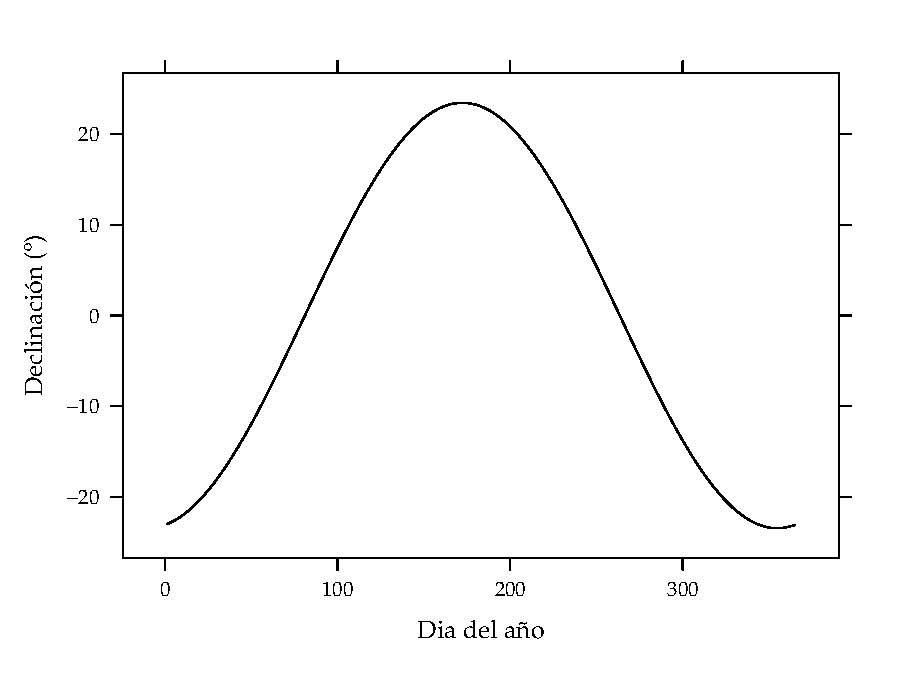
\includegraphics[width=.9\linewidth]{../figs/Declinacion.pdf}
\end{center}
\end{frame}

\begin{frame}[label={sec:org70460b5}]{Otras ecuaciones}
\begin{center}
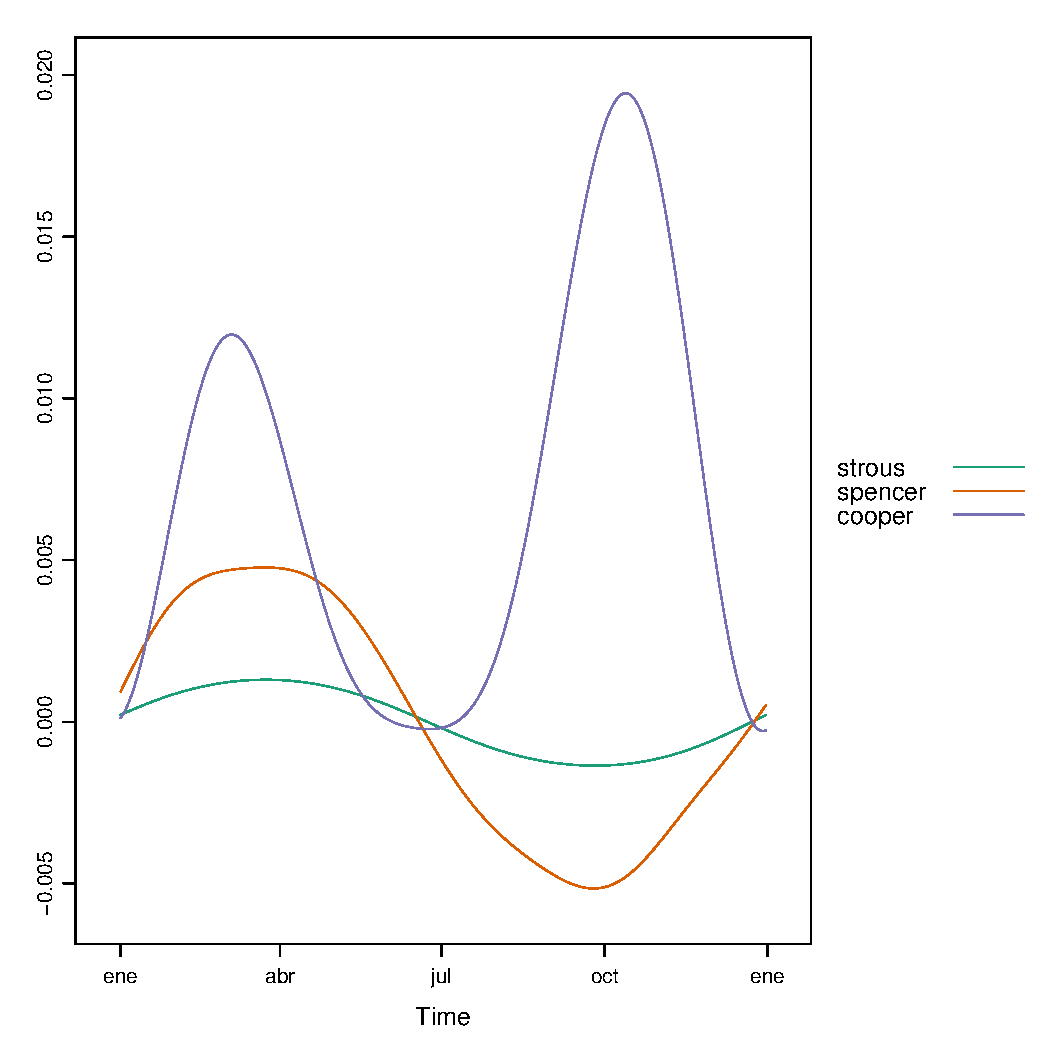
\includegraphics[width=.9\linewidth]{../figs/DeclinacionDiferencias.pdf}
\end{center}
\end{frame}

\subsection{Sistemas de coordenadas}
\label{sec:org1b9e484}

\begin{frame}[label={sec:org9386545}]{Ejes terrestres}
\begin{center}
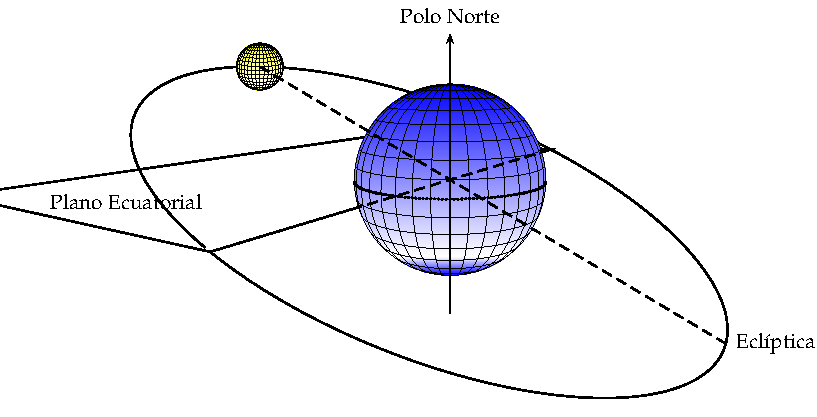
\includegraphics[width=.9\linewidth]{../figs/SoldesdeTierra.pdf}
\end{center}

\[\vec{\mu}_{s}=\left[\cos\left(\delta\right)\cos\left(\omega\right)\right]\cdot\vec{\mu}_{ec}+\left[\cos\left(\delta\right)\sin\left(\omega\right)\right]\cdot\vec{\mu}_{\bot}+\sin\left(\delta\right)\cdot\vec{\mu}_{p}\]
\end{frame}



\begin{frame}[label={sec:org174ea23}]{Ejes terrestres}
\begin{center}
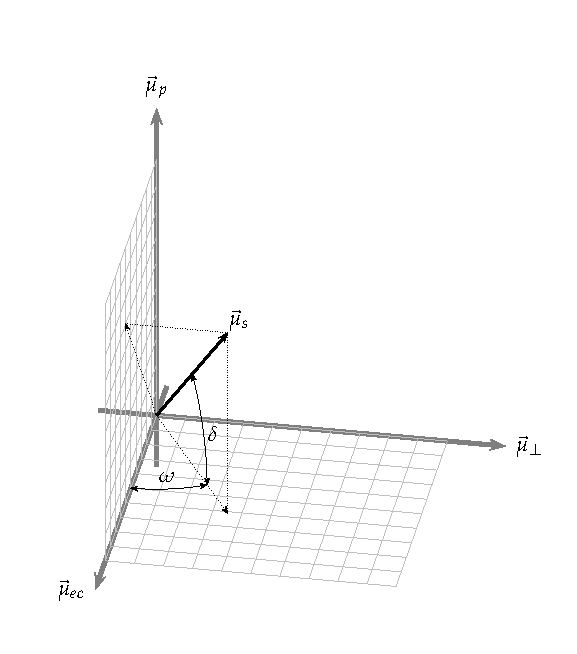
\includegraphics[height=0.7\textheight]{../figs/SistemaCoordenadasTerrestre.pdf}
\end{center}


\[\vec{\mu}_{s}=\left[\cos\left(\delta\right)\cos\left(\omega\right)\right]\cdot\vec{\mu}_{ec}+\left[\cos\left(\delta\right)\sin\left(\omega\right)\right]\cdot\vec{\mu}_{\bot}+\sin\left(\delta\right)\cdot\vec{\mu}_{p}\]
\end{frame}


\begin{frame}[label={sec:orgc8a26f2}]{Ejes locales}
\begin{center}
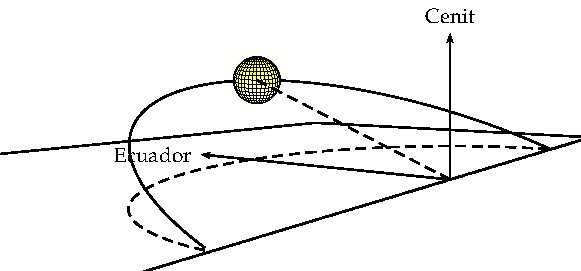
\includegraphics[width=.9\linewidth]{../figs/SoldesdeTierra2.pdf}
\end{center}

\[\vec{\mu}_{s}=\left[\cos\left(\psi_{s}\right)\sin\left(\theta_{z}\right)\right]\cdot\vec{\mu}_{h}+\left[\sin\left(\psi_{s}\right)\sin\left(\theta_{z}\right)\right]\cdot\vec{\mu}_{\bot}+\cos\left(\theta_{z}\right)\cdot\vec{\mu}_{c}\]
\end{frame}



\begin{frame}[label={sec:org13e4ccb}]{Ejes locales}
\begin{center}
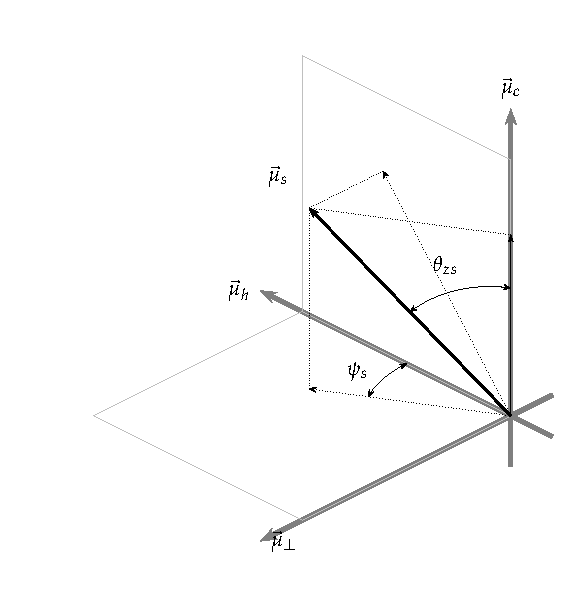
\includegraphics[width=.9\linewidth]{../figs/SistemaCoordenadasLocal.pdf}
\end{center}

\[\vec{\mu}_{s}=\left[\cos\left(\psi_{s}\right)\sin\left(\theta_{z}\right)\right]\cdot\vec{\mu}_{h}+\left[\sin\left(\psi_{s}\right)\sin\left(\theta_{z}\right)\right]\cdot\vec{\mu}_{\bot}+\cos\left(\theta_{z}\right)\cdot\vec{\mu}_{c}\]
\end{frame}

\begin{frame}[label={sec:orga122a4f}]{Relación entre sistemas de coordenadas}
\begin{center}
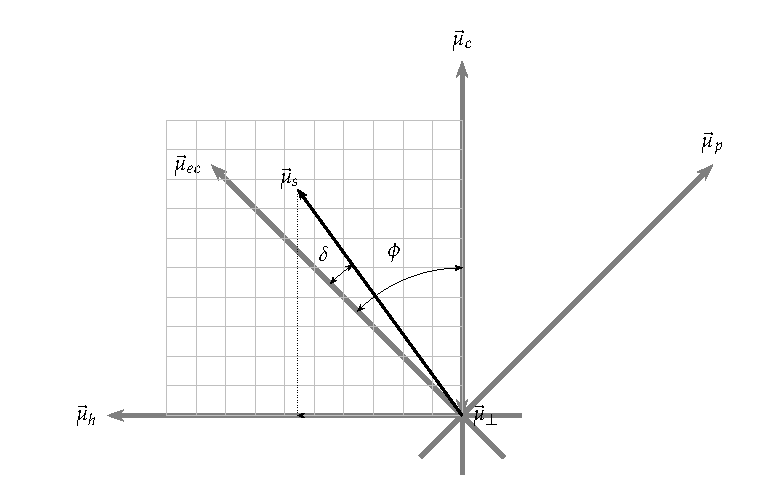
\includegraphics[width=.9\linewidth]{../figs/RelacionSistemasCoordenadas.pdf}
\end{center}
\end{frame}

\begin{frame}[label={sec:orge7e4997}]{Ejes locales y terrestres}
\begin{align*}
  \vec{\mu}_{s} &= \mathrm{signo}(\phi)\cdot\left[\cos\left(\delta\right)\cos\left(\omega\right)\sin\left(\phi\right)-\cos\left(\phi\right)\sin\left(\delta\right)\right]\cdot\vec{\mu}_{h}-\\
  &- \left[\cos\left(\delta\right)\sin\left(\omega\right)\right]\cdot\vec{\mu}_{\bot}+\\
  &+ \left[\cos\left(\delta\right)\cos\left(\omega\right)\cos\left(\phi\right)+\sin\left(\delta\right)\sin\left(\phi\right)\right]\cdot\vec{\mu}_{c} 
\end{align*}


\alert{Latitud (\(\phi\)) con signo}: Positivo para Hemisferio Norte, Negativo para Hemisferio Sur.
\end{frame}

\subsection{Ángulos Solares}
\label{sec:org2ac1cc8}

\begin{frame}[label={sec:org6cc83ab}]{Ecuaciones}
\begin{block}{Cenit solar}
\[\cos\left(\theta_{z}\right)=\vec{\mu}_{c}\cdot\vec{\mu}_{s}=\cos\left(\delta\right)\cos\left(\omega\right)\cos\left(\phi\right)+\sin\left(\delta\right)\sin\left(\phi\right)\]
\end{block}

\begin{block}{Azimut solar}
\begin{align*}
  \vec{\mu_{s}}\cdot\vec{\mu}_{\bot} &=-\sin\left(\psi_{s}\right)\sin\left(\theta_{zs}\right)\\
  \vec{\mu_{s}}\cdot\vec{\mu}_{h} &=\mathrm{signo}(\phi)\cdot\cos\left(\psi_{s}\right)\sin\left(\theta_{zs}\right)\\
  \cos\left(\psi_{s}\right) &= \mathrm{signo}(\phi)\cdot\frac{\cos\left(\delta\right)\cos\left(\omega\right)\sin\left(\phi\right)-\cos\left(\phi\right)\sin\left(\delta\right)}{\sin\left(\theta_{zs}\right)}\\
  \sin(\psi_{s}) &=\frac{\cos(\delta)\sin(\omega)}{\sin(\theta_{zs})}=\frac{\cos(\delta)\sin(\omega)}{\cos(\gamma_{s})}
\end{align*}
\end{block}
\end{frame}



\begin{frame}[label={sec:orgeb660e6}]{Trayectoria Solar (\(60\degree N\))}
\begin{center}
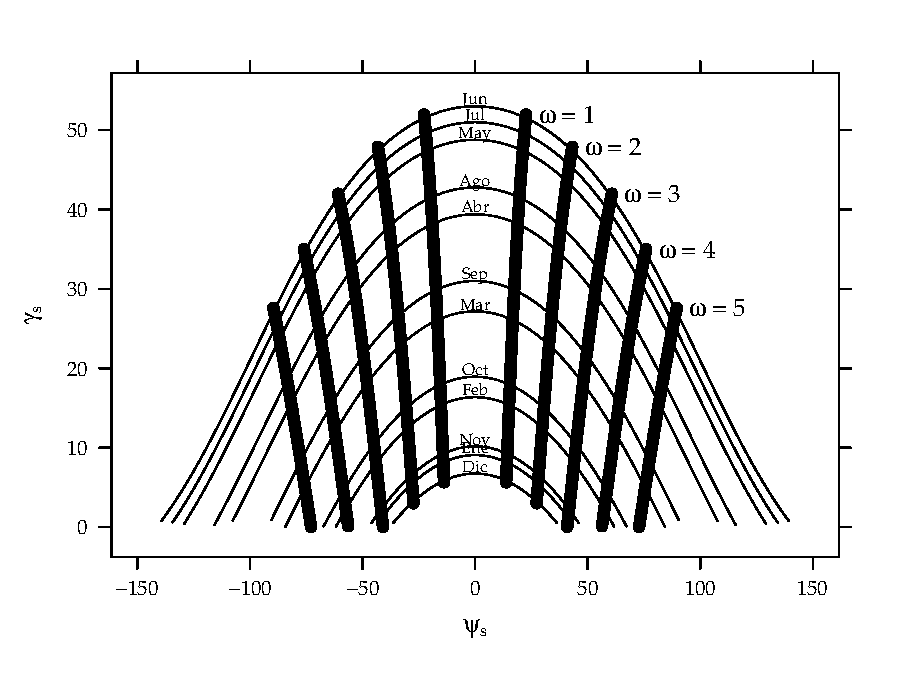
\includegraphics[width=.9\linewidth]{../figs/TrayectoriaSolar60N.pdf}
\end{center}
\end{frame}



\begin{frame}[label={sec:orgc51f6b9}]{Trayectoria Solar (\(40\degree S\))}
\begin{center}
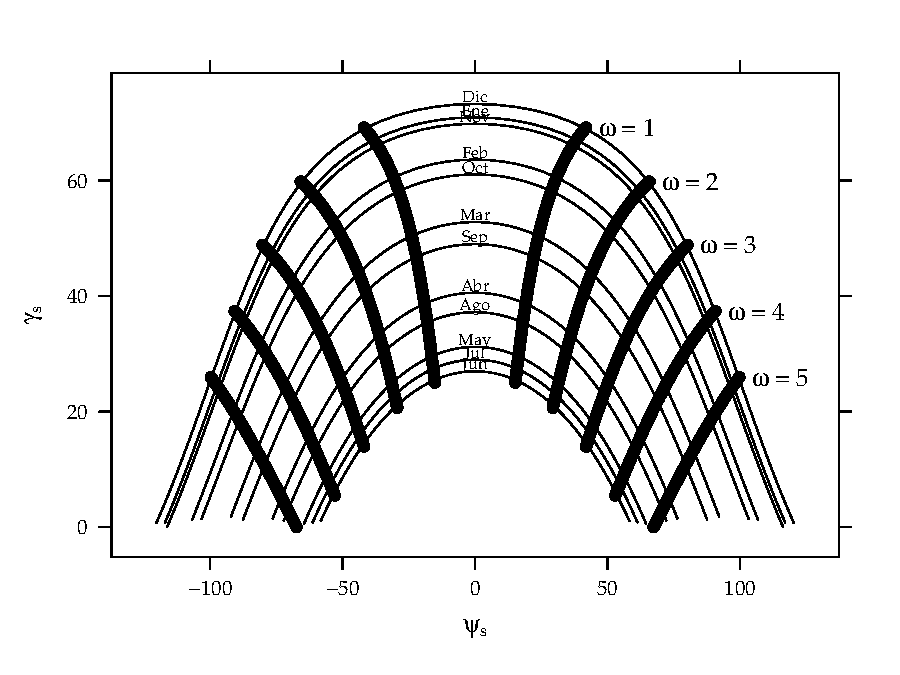
\includegraphics[width=.9\linewidth]{../figs/TrayectoriaSolar40S.pdf}
\end{center}
\end{frame}


\begin{frame}[label={sec:orgc877635}]{Mediodía, amanecer y anocher}
\begin{itemize}
\item Mediodía: \[\psi_{s}=0\Rightarrow\sin(\psi_{s})\Rightarrow\omega=0\]

\item Amanecer / Anochecer:
\[\gamma_{s}=0,\,\theta_{z}=\frac{\pi}{2}\Rightarrow\cos(\theta_{z})=0\]
\end{itemize}
\[\cos(\omega_{s})=-\tan(\delta)\tan(\phi)\]
\end{frame}

\begin{frame}[label={sec:org0891361}]{Duración del día}
\begin{center}
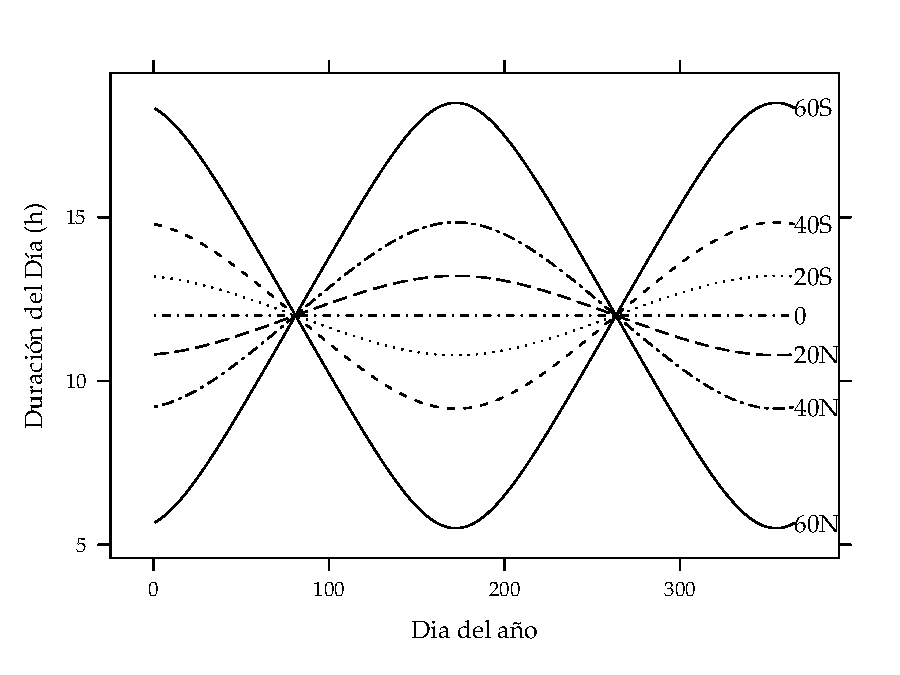
\includegraphics[width=.9\linewidth]{../figs/DuracionDia.pdf}
\end{center}
\end{frame}

\begin{frame}[label={sec:org907f66c}]{Cálculo Ángulos Solares}
\begin{itemize}
\item Azimut, Ángulo Cenital y Altura Solar, Duración del Dia para el:

\begin{itemize}
\item Día del Año: 120, 2 horas después del mediodía, Latitud: 37.2N

\item Día del Año: 340, 2 horas después del amanecer, Latitud: 15S
\end{itemize}

\item Duración del día 261 del año en las latitudes 10N, 40N, 70N, 10S,
40S, 70S.

\item Altura solar en el mediodía del día 25 del año en las latitudes 10N,
40N, 10S, 40S.
\end{itemize}
\end{frame}

\subsection{Hora solar y oficial}
\label{sec:orgd939151}
\begin{frame}[label={sec:orgc732321}]{Hora solar}
\[\omega=15\cdot(\mathrm{TO}-\mathrm{AO}-12)+\Delta\lambda+\frac{\mathrm{EoT}}{4}\]

\begin{itemize}
\item \(\omega\): hora solar real o aparente[º]
\item \(TO\): hora oficial [h]
\item \(AO\): adelanto oficial por horario de verano [h]
\item \(\Delta\lambda\) corrección por huso horario [º]
\item \(EoT\): Ecuación del tiempo (dia solar real y dia solar medio) [min]
\end{itemize}
\end{frame}

\begin{frame}[label={sec:orgdd5d113}]{Hora oficial}
\begin{itemize}
\item \alert{La hora oficial} es una medida del tiempo \alert{ligada a un meridiano}
que sirve de referencia para una zona determinada.

\item La hora oficial de la España peninsular se rija por el huso horario
de Centroeuropa. Este huso horario está situado en
\(15\degree\mathrm{E}\).
\end{itemize}
\end{frame}

\begin{frame}[label={sec:org6c6b9e4}]{Hora oficial}
\begin{itemize}
\item \alert{Corrección}: \(\Delta\lambda=\lambda_{L}-\lambda_{H}\), con
\(\lambda_{L}\) la longitud local y \(\lambda_{H}\) la longitud del huso
horario.

\item Longitudes \emph{positivas} al \emph{este} del meridiano de Greenwich.
\(\Delta\lambda\) es positiva cuando la localidad está situada al este
de su huso horario.

\item Diferencia adicional: \emph{horario de verano}.
\end{itemize}
\end{frame}

\begin{frame}[label={sec:org3206be0}]{Tiempo solar medio}
\begin{itemize}
\item \alert{La duración del día solar real}, definido como el tiempo que
transcurre entre dos pasos consecutivos del Sol por el meridiano
local, \alert{varía a lo largo del año}.

\item El promedio anual de esta variación es nulo: \emph{día solar medio}, cuya
duración es constante a lo largo del año e igual al valor medio de la
duración del día solar real.
\end{itemize}
\end{frame}

\begin{frame}[label={sec:org7d38e25}]{Ecuación del Tiempo}
\(\mathrm{EoT}=229.18\cdot\left(-0.0334\cdot\sin(M)+0.04184\cdot\sin\left(2\cdot
      M+3.5884\right)\right)\)

\begin{center}
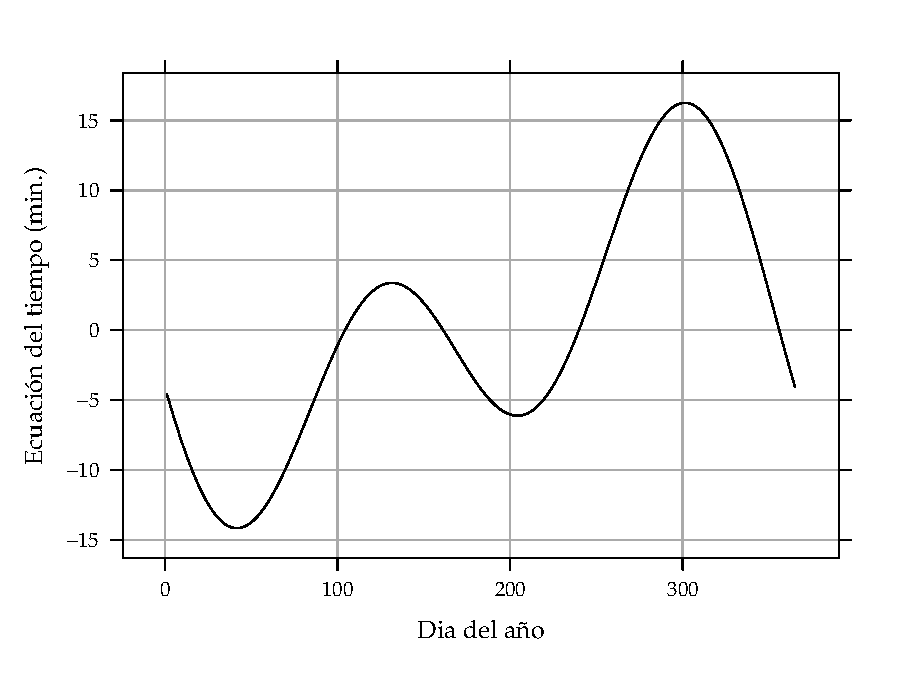
\includegraphics[width=.9\linewidth]{../figs/EoT.pdf}
\end{center}
\end{frame}

\begin{frame}[label={sec:org79083e4}]{Ejemplo de cálculo}
\[\omega=15\cdot(\mathrm{TO}-\mathrm{AO}-12)+\Delta\lambda+\frac{\mathrm{EoT}}{4}\]

\begin{block}{}
Calcule la hora solar real correspondiente al día 23 de Abril de 2010
  (\(\mathrm{EoT=\SI{1.78}{\minute}}\)) a las 12 de la mañana, hora
  oficial de la ciudad de A Coruña, Galicia. Esta localidad está
  contenida en el meridiano de longitud \(8.38\degree\mathrm{W}\) y su
  hora oficial está regida por el huso horario GMT+1.
\end{block}
\end{frame}

\begin{frame}[label={sec:org3849748}]{Solución}
\[\omega=15\cdot(\mathrm{TO}-\mathrm{AO}-12)+\Delta\lambda+\frac{\mathrm{EoT}}{4}\]

\begin{itemize}[<+->]
\item \(\lambda_{L}=-8.38\degree\), \(\lambda_{H}=15\degree\) y
\(\Delta\lambda=-23.38\degree\).

\item En España se aplica el horario de verano y este día está incluido
en el período afectado, \(\mathrm{AO}=1\).

\item Por último, para este día \(\mathrm{EoT=\SI{1.78}{\minute}}\).

\item Así \(\omega=-37.94\degree\) (aproximadamente las 9 y media de la
mañana). El Sol culminará (\(\omega=0\)) cuando sean las 14:31, hora
oficial.
\end{itemize}
\end{frame}


\section{Geometría de los sistemas fotovoltaicos}
\label{sec:orge544bf0}

\subsection{Sistemas Estáticos y de Seguimiento}
\label{sec:org357a0e4}
\begin{frame}[label={sec:orge8ef2f6}]{Sistemas estáticos}
\begin{center}
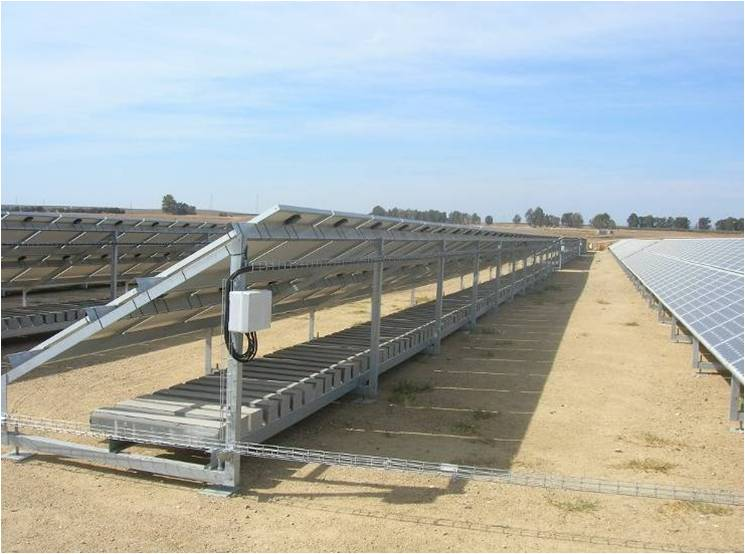
\includegraphics[width=.9\linewidth]{../figs/EstructuraEstaticaSuelo.jpg}
\end{center}
\end{frame}

\begin{frame}[label={sec:orgf9ecd70}]{Sistemas con seguimiento}
\begin{itemize}[<+->]
\item \alert{Fundamento:}
\begin{itemize}[<.->]
\item Radiación incidente aumenta al seguir al sol

\item Pérdidas por reflexión disminuyen si el apuntamiento al sol mejora
\end{itemize}

\item Las diferentes técnicas de seguimiento son un compromiso entre un
apuntamiento perfecto y sistemas estructurales más económicos y
mejores aprovechamientos del terreno.
\end{itemize}
\end{frame}

\begin{frame}[label={sec:org1e51bf9}]{Algunos tipos de seguimiento solar}
\begin{itemize}[<+->]
\item \alert{Doble eje}
\begin{itemize}[<.->]
\item Apuntamiento \guillemotleft{}perfecto\guillemotright{}

\item Mejor productividad, peor ocupación de terreno.
\end{itemize}

\item \alert{Seguimento acimutal}
\begin{itemize}[<.->]
\item Sacrifica un movimiento (inclinación del generador) para conseguir
sistemas más económicos.
\end{itemize}

\item \alert{Seguimiento horizontal con eje Norte-Sur}
\begin{itemize}[<.->]
\item Sencillez y estabilidad estructural (el eje es horizontal y
paralelo al terreno, con tantos puntos de apoyo como se consideren
necesarios),

\item Facilidad de motorización,

\item Buen aprovechamiento del terreno.
\end{itemize}
\end{itemize}
\end{frame}


\begin{frame}[label={sec:orgf92e18a}]{Seguidor de eje horizontal N-S}
\begin{center}
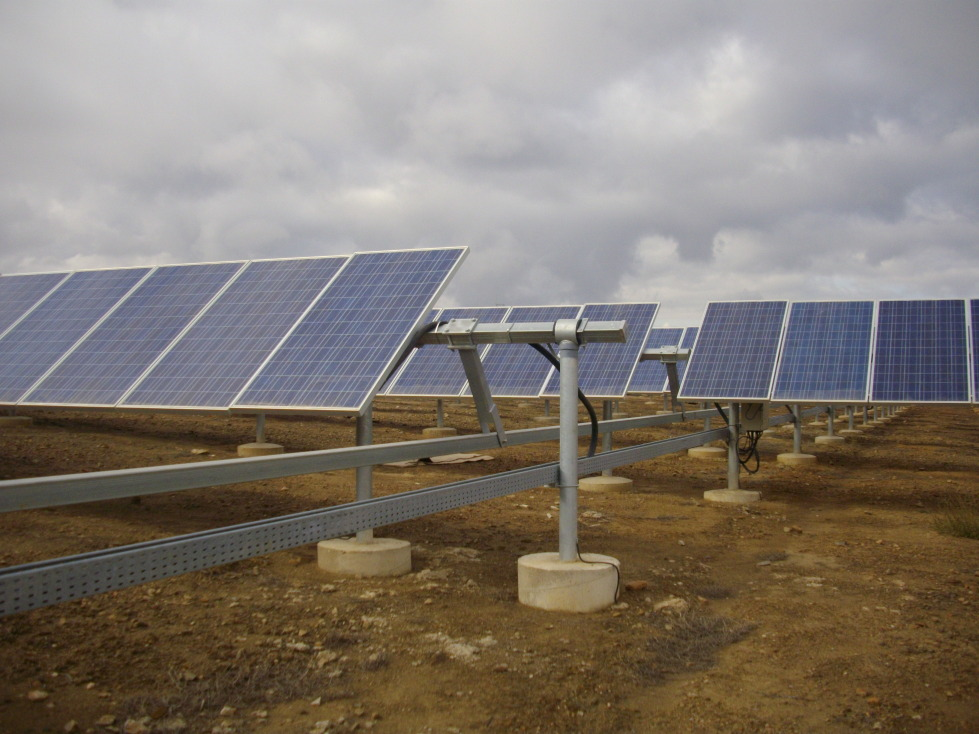
\includegraphics[width=.9\linewidth]{../figs/SeguidorEjeHorizontal.jpg}
\end{center}
\end{frame}


\begin{frame}[label={sec:org9268ccf}]{Seguidor de doble eje}
\begin{center}
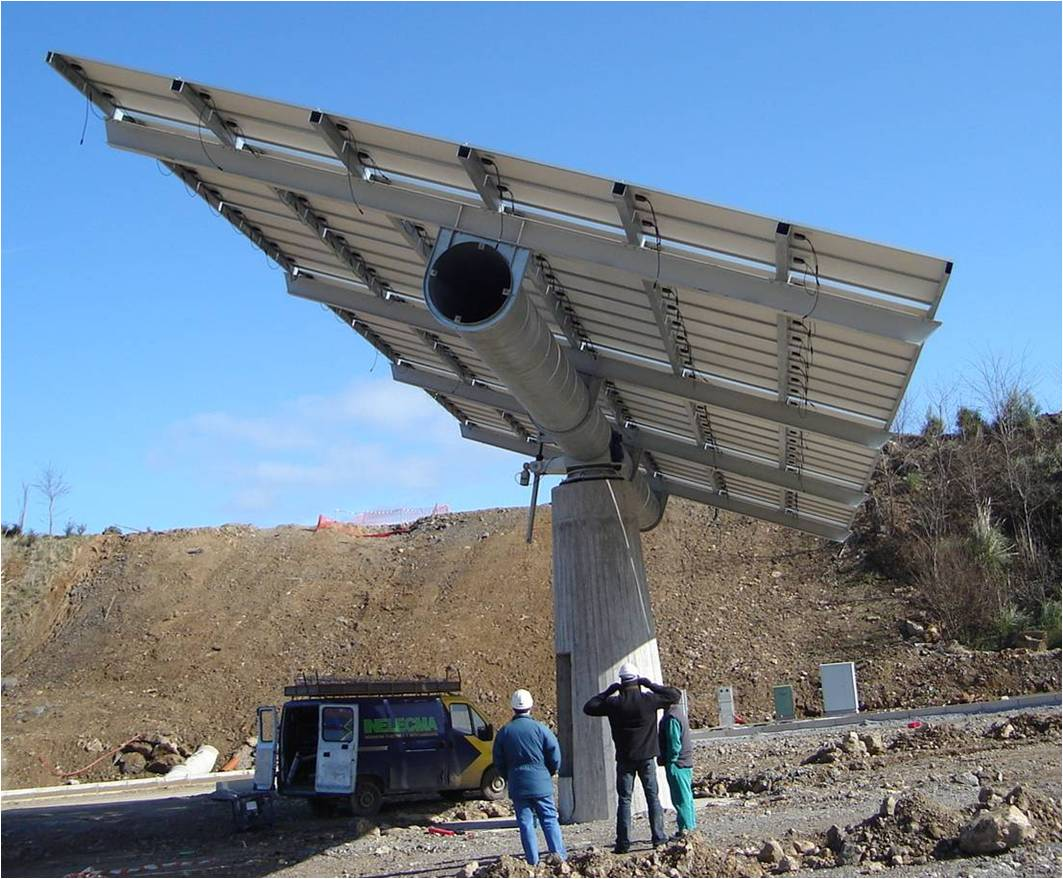
\includegraphics[width=.9\linewidth]{../figs/SeguidorReocin.jpg}
\end{center}
\end{frame}


\subsection{Ángulos}
\label{sec:org834f549}

\begin{frame}[label={sec:org6a9a452}]{Sistema Estático}
\begin{itemize}
\item Vector de posición
\end{itemize}
\[\vec{\mu}_{\beta}=[\sin(\beta)\cos(\alpha)]\cdot\vec{\mu}_{h}+[\sin(\beta)\sin(\alpha)]\cdot\vec{\mu}_{\bot}+\cos(\beta)\cdot\vec{\mu}_{c}\]

\begin{center}
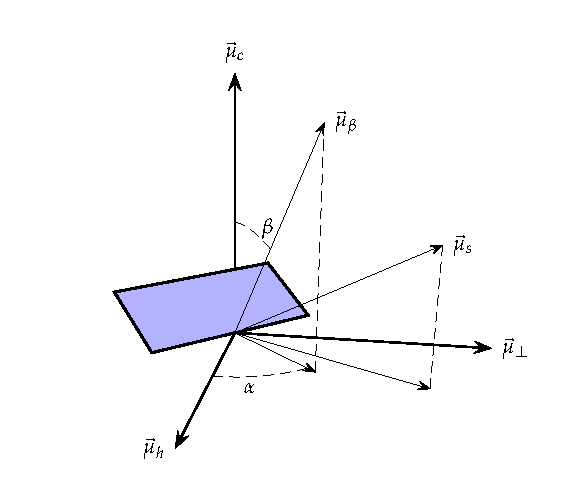
\includegraphics[width=.9\linewidth]{../figs/AngulosSistemaEstatico.pdf}
\end{center}
\end{frame}

\begin{frame}[label={sec:orgf64084b}]{Sistema Estático}
\begin{itemize}
\item Ángulo de Incidencia
\end{itemize}

\begin{align*}
\cos(\theta_{s}) &= \mathrm{signo}(\phi)\cdot\bigl[\sin(\beta)\cos(\alpha)\cos\left(\delta\right)\cos\left(\omega\right)\sin\left(\phi\right)-\\
 &- \sin(\beta)\cos(\alpha)\cos\left(\phi\right)\sin\left(\delta\right)\bigr]+\\
 &+ \sin(\beta)\sin(\alpha)\cos\left(\delta\right)\sin\left(\omega\right)+ \\
 &+ \cos(\beta)\cos\left(\delta\right)\cos\left(\omega\right)\cos\left(\phi\right)+\\
 &+ \cos(\beta)\sin\left(\delta\right)\sin\left(\phi\right)
\end{align*}


\begin{center}
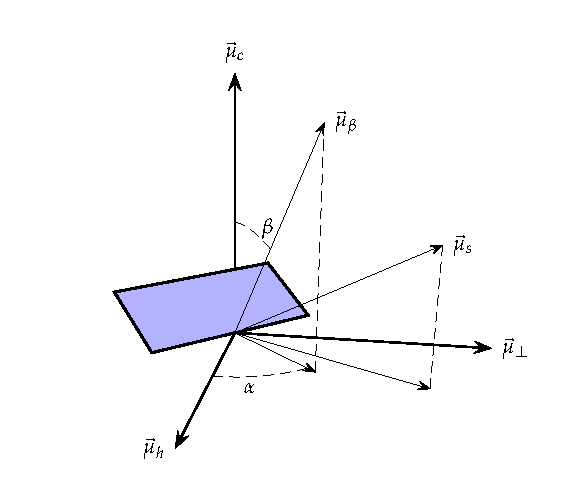
\includegraphics[height=0.4\textheight]{../figs/AngulosSistemaEstatico.pdf}
\end{center}
\end{frame}


\begin{frame}[label={sec:orgef183ee}]{Sistema Estático}
Cuando \(\alpha=0\)

\begin{align*}
\cos(\theta_{s}) &= \cos\left(\delta\right)\cos\left(\omega\right)\cos\left(\beta-|\phi|\right)-\\ 
&- \mathrm{signo}(\phi)\cdot\sin(\delta)\sin\left(\beta-|\phi|\right)
\end{align*}


\begin{center}
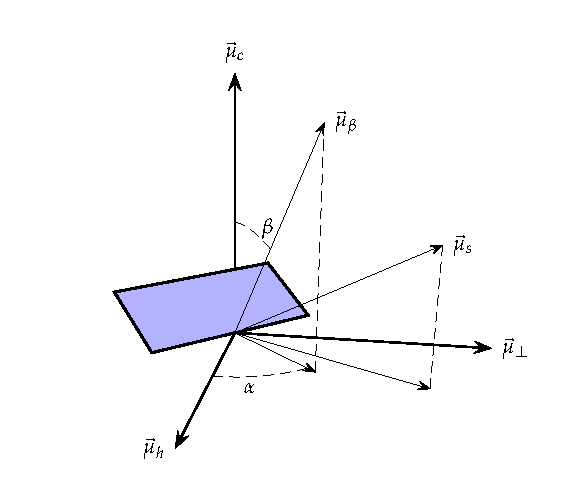
\includegraphics[height=0.6\textheight]{../figs/AngulosSistemaEstatico.pdf}
\end{center}
\end{frame}


\begin{frame}[label={sec:org34ae814}]{Ángulo de Incidencia de Sistema Estático}
\begin{itemize}
\item \(40\degree N\)
\end{itemize}
\begin{center}
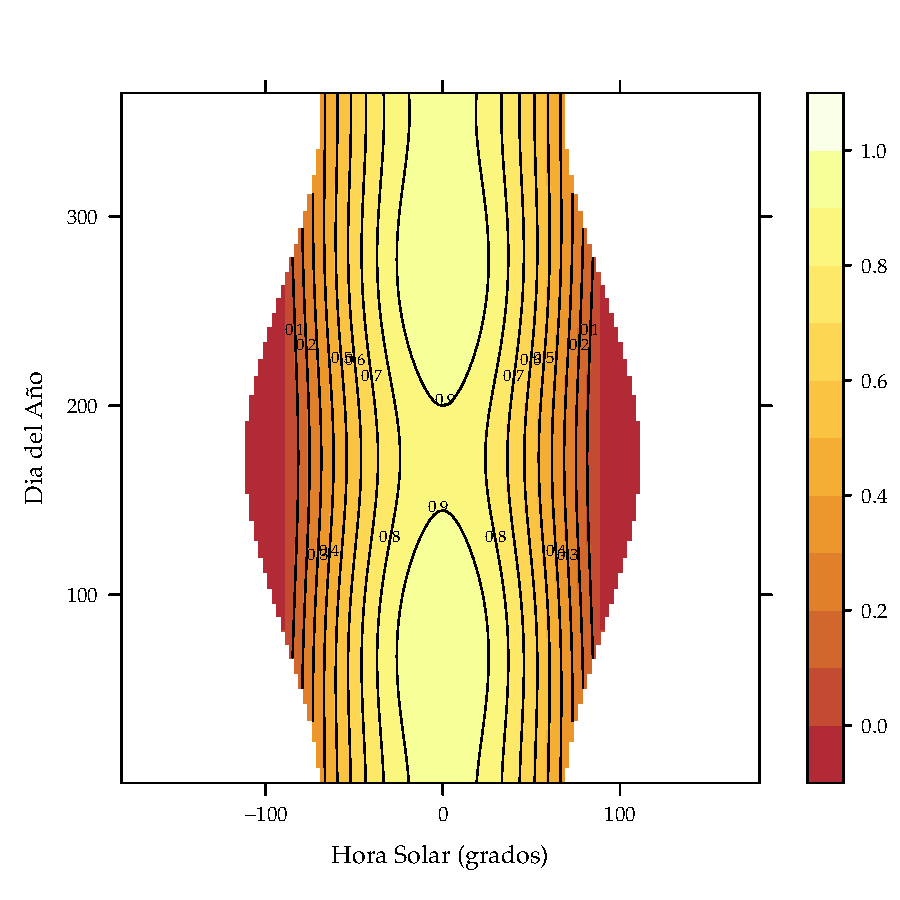
\includegraphics[height=0.8\textheight]{../figs/cosThetaEst_40N.pdf}
\end{center}
\end{frame}



\begin{frame}[label={sec:orgebd8b6d}]{Eje Horizontal N-S, generador horizontal}
\begin{itemize}
\item Vector de posición
\end{itemize}

\[\vec{\mu}_{ns}=\sin(\psi_{ns})\cdot\vec{\mu}_{\bot}+\cos(\psi_{ns})\cdot\vec{\mu}_{c}\]

\begin{center}
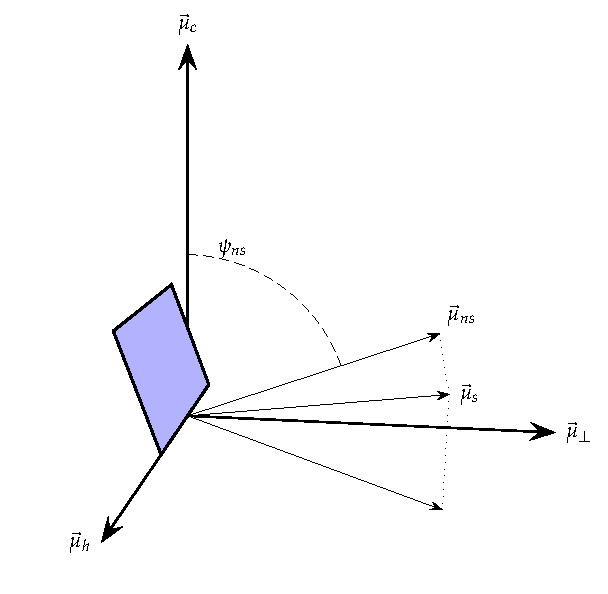
\includegraphics[height=0.6\textheight]{../figs/AngulosSistemaHorizontalNS.pdf}
\end{center}
\end{frame}



\begin{frame}[label={sec:orgf3706bb}]{Eje Horizontal N-S, generador horizontal}
\begin{itemize}
\item Ángulo de Incidencia
\end{itemize}

\[\cos(\theta_{s})=\cos(\delta)\sqrt{\sin^{2}(\omega)+\left(\cos(\omega)\cos(\phi)+\tan(\delta)\sin(\phi)\right)^{2}}\]

\begin{center}
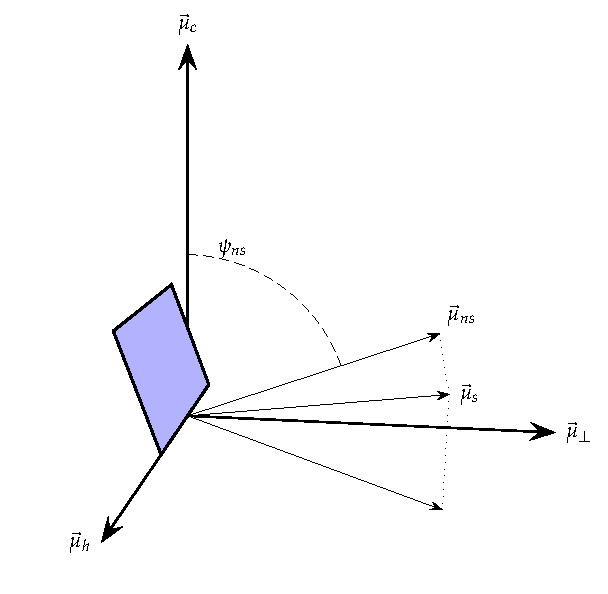
\includegraphics[height=0.6\textheight]{../figs/AngulosSistemaHorizontalNS.pdf}
\end{center}
\end{frame}


\begin{frame}[label={sec:orgfaf061a}]{Inclinación de Eje Horizontal N-S}
\begin{itemize}
\item \(40\degree N\)
\end{itemize}
\begin{center}
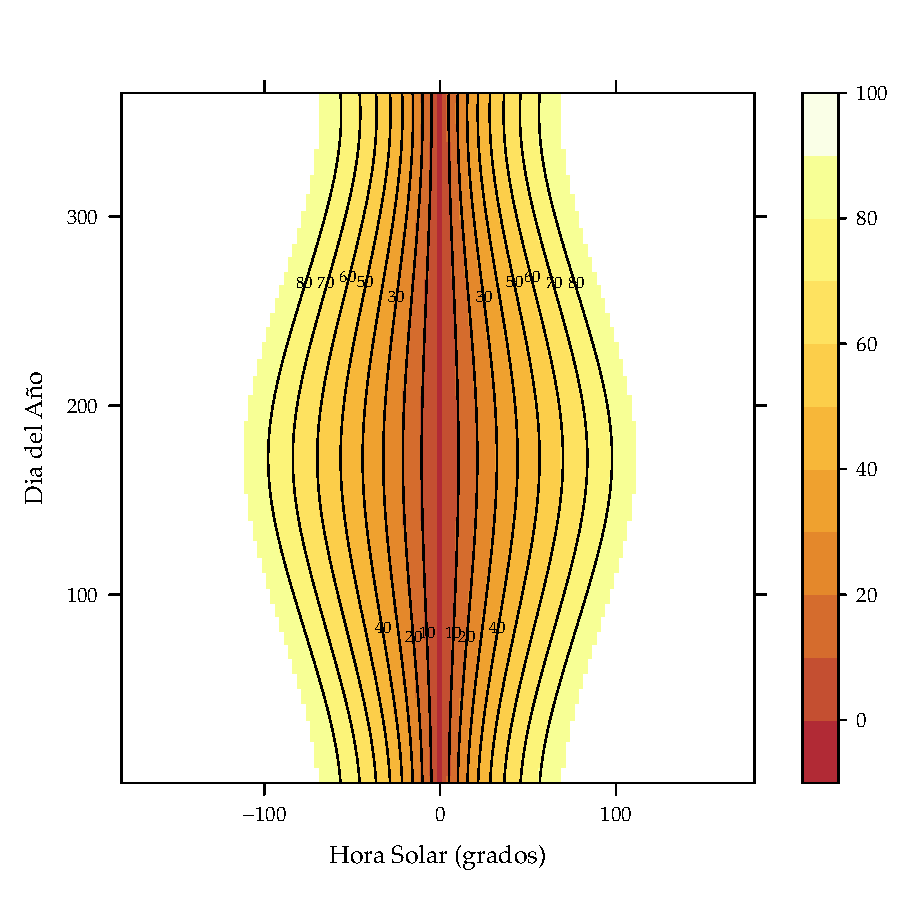
\includegraphics[height=0.8\textheight]{../figs/BetaHoriz_40N.pdf}
\end{center}
\end{frame}



\begin{frame}[label={sec:orgd1e54d5}]{Ángulo de Incidencia de Eje Horizontal N-S}
\begin{itemize}
\item \(40\degree N\)
\end{itemize}
\begin{center}
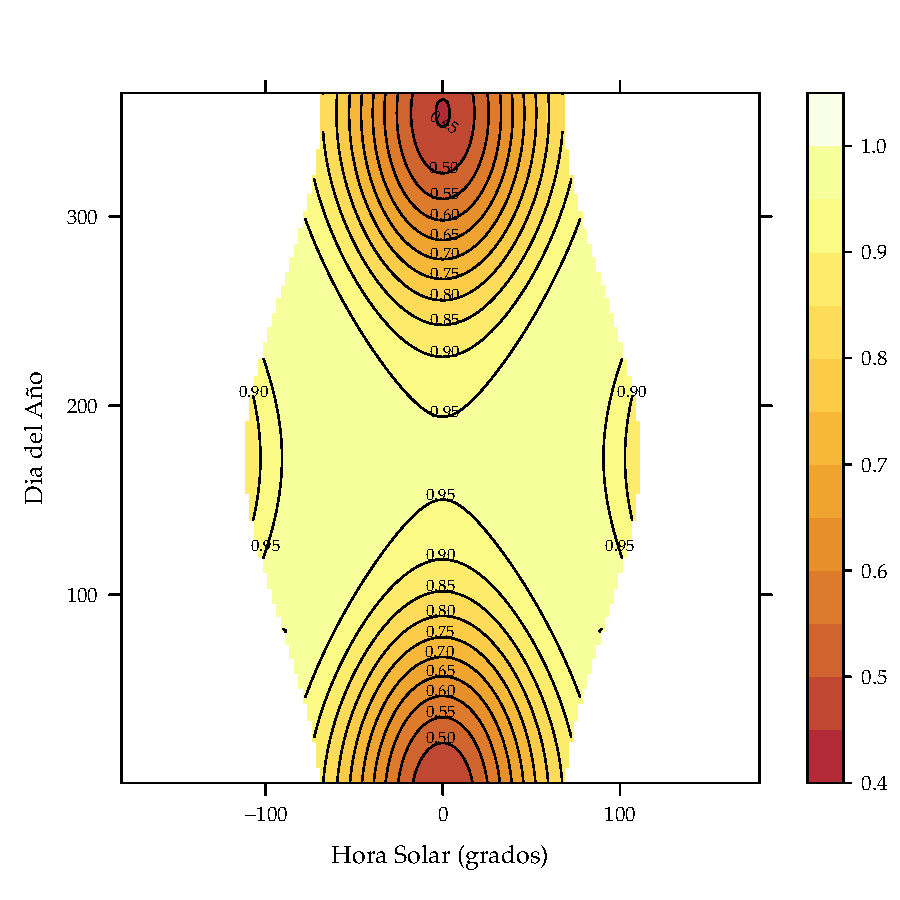
\includegraphics[height=0.8\textheight]{../figs/cosThetaHoriz_40N.pdf}
\end{center}
\end{frame}


\begin{frame}[label={sec:org9f90fa3}]{Acimutal}
\begin{center}
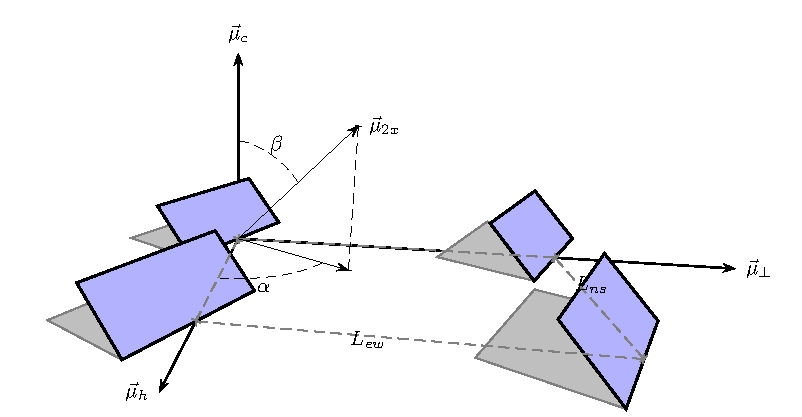
\includegraphics[width=.9\linewidth]{../figs/Sombra2X.pdf}
\end{center}


\begin{align*}
  \beta &= cte.\\
  \alpha &= \psi_{s}\\
  \cos(\theta_{s}) &= \cos\left(\beta-\theta_{z}\right)
\end{align*}
\end{frame}




\begin{frame}[label={sec:org037aee1}]{Orientación de un seguidor acimutal}
\begin{itemize}
\item \(40\degree N\)
\end{itemize}
\begin{center}
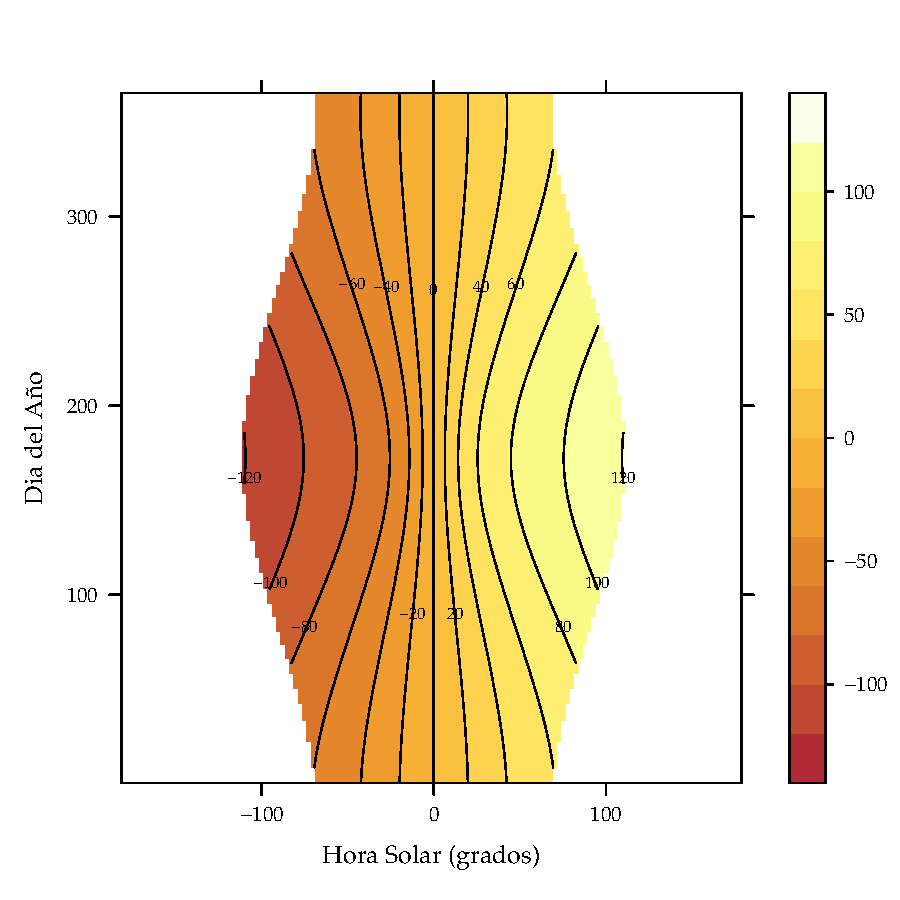
\includegraphics[height=0.8\textheight]{../figs/AlfaDoble_40N.pdf}
\end{center}
\end{frame}

\begin{frame}[label={sec:org26ac210}]{Ángulo de Incidencia en Acimutal}
\begin{itemize}
\item \(40\degree N\)
\end{itemize}
\begin{center}
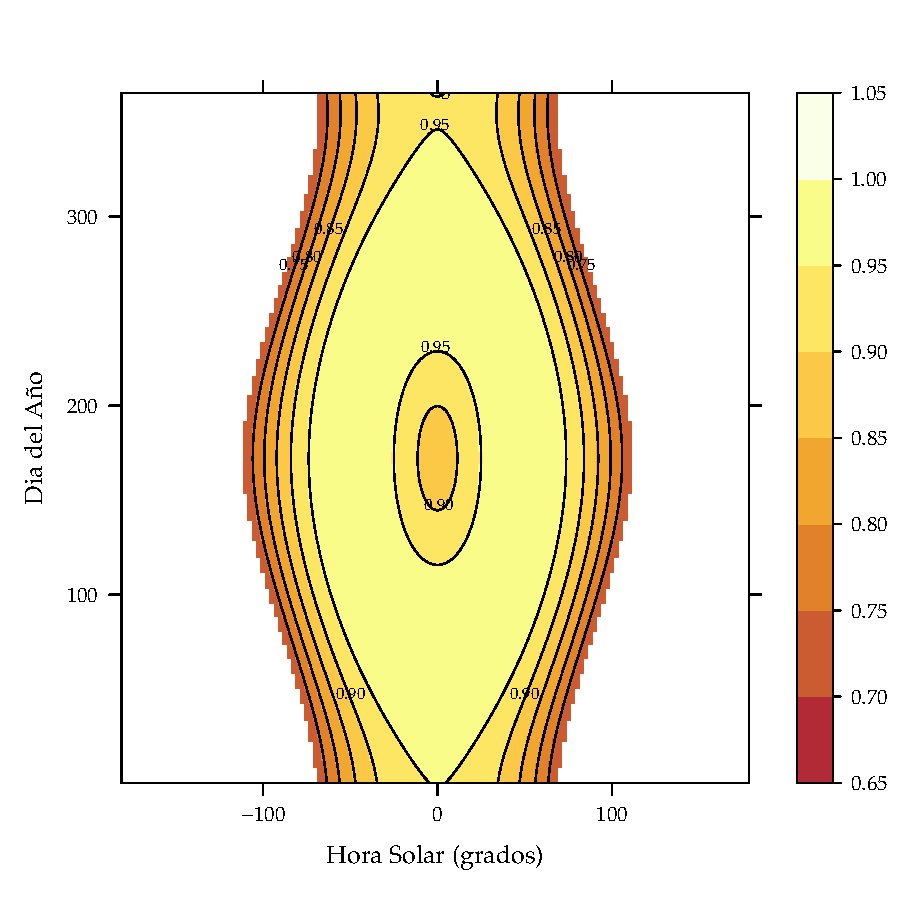
\includegraphics[height=0.8\textheight]{../figs/cosThetaAzimutal_40N.pdf}
\end{center}
\end{frame}


\begin{frame}[label={sec:org874fe60}]{Doble Eje}
\begin{center}
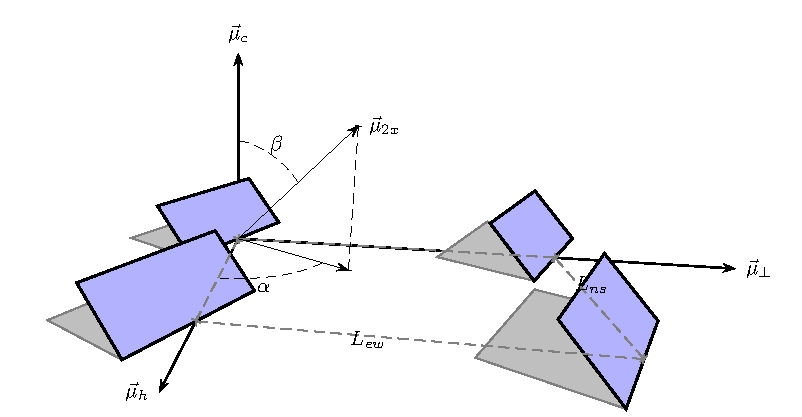
\includegraphics[width=.9\linewidth]{../figs/Sombra2X.pdf}
\end{center}


\begin{align*}
  \beta &= \theta_{z}\\
  \alpha &= \psi_{s}\\
  \cos(\theta_{s}) &= 1
\end{align*}
\end{frame}



\begin{frame}[label={sec:orgeadb2f7}]{Inclinación de un seguidor de Doble Eje}
\begin{itemize}
\item \(40\degree N\)
\end{itemize}
\begin{center}
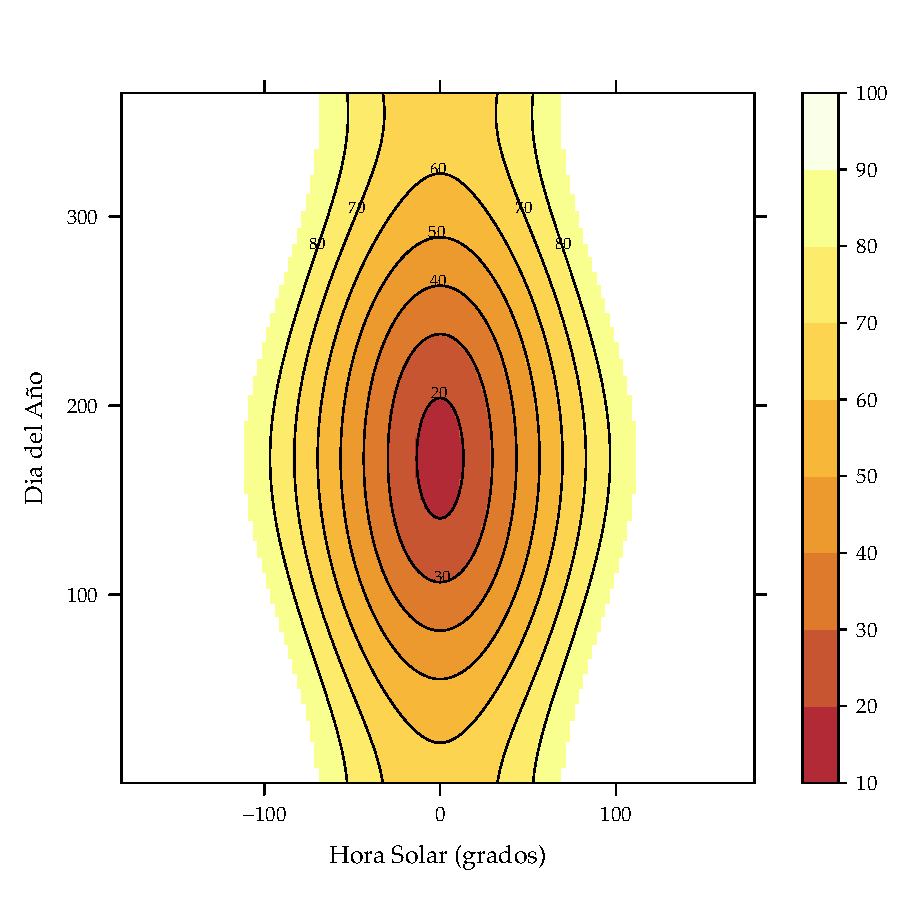
\includegraphics[height=0.8\textheight]{../figs/BetaDoble_40N.pdf}
\end{center}
\end{frame}



\begin{frame}[label={sec:orgf940f80}]{Ejercicio: cálculo de ángulo de incidencia}
\begin{description}
\item[{Para:}] \begin{itemize}
\item Un sistema estático orientado al Sur y con inclinación de 30;

\item Un sistema de seguimiento horizontal N-S;

\item Un sistema de seguimiento acimutal con inclinación a 35;

\item Un sistema de seguimiento a doble eje,
\end{itemize}

\item[{Calcular}] el ángulo de incidencia para el:

\begin{itemize}
\item Día del Año: 120, 2 horas después del mediodía, Latitud: 37.2N;

\item Día del Año: 340, 2 horas después del amanecer, Latitud: 15S;
\end{itemize}
\end{description}
\end{frame}
\end{document}